
\subsection{Software Performance And HPC Architecture}
\label{subsec:hpc}

For a specific algorithm with a given data size, numbers of elemental operations, such as floating point operation, data copy between memory and CPU, data copy between memories in different nodes, necessary to execute the simulation can be estimated. Here, we assume that our interests are rather on large  scale simulations with large size of data where memory bandwidth become more important than cache. If one compares the ratio between those operations with the hardware specification of a HPC system one can obtain an insight as to which operation is likely to become the limiting factor for the overall performance of the simulation on a given HPC system. 

For instance, the performance behavior of parallel 3D FFT, which occupies significant portion of computational time in a GGA/LDA level DFT simulation, on HPC system has been studied extensively and it is known that interconnect bandwidth (IB) as well as memory bandwidth (MB) are more important factors for a good performance than flops count (FP) owing to the nature of algorithm: Cooley-Tukey algorithm that takes full advantage of the structure of operation and minimize the number of floating point operation leading to dramatic decrease in the computational cost and improving its scaling from $N^2$ to $N\log{N}$.\cite{cooley1965} Here, $N$ is the FFT grid size.

This, combined with the dual space formalism,\cite{Martin1988} played a critical role for the widespread use of planewave pseudopotential density functional theory simulations in the scientific community. However, the fact that the operation has to be performed on the entire data set does not change even with the revolutional FFT algorithm leading to the bottleneck being data moves either between CPU and memory or between memories on different nodes. Accordingly, it is very likely that the IB becomes the performance limiting factor of parallel 3D FFT as well as GGA level DFT on the currently available CPU-GPU hydbrid HPC systems such as Sierra (LLNL) and Summit (ORNL), which largely share GPU and interconnect specifications. 

\begin{table}[ht]
    \centering
    \begin{tabular}{|l|lll|}
    \hline
        Machine (institute) &  MB/flops & IB/flops & IB/flops \\
        \hline
        Sierra (LLNL) &  0.1 byte/flops & 0.0036 byte/flops & 0.025 \\
        Quartz (LLNL) & 0.154 byte/flops & 0.048 byte/flops & 0.156\\
        Fugaku (Riken) &  0.3 byte/flops & 0.014 byte/flops  & 0.041 \\
        \hline
    \end{tabular}
    \caption{HPC system parameters relevant for data access intensive algorithm such as FFT for a few currently active HCP systems. For the scaling of memory access intensive algorithms may be rather dictated by IB/MB since the serial performance is dictated by MB not FP.}
    \label{tab:hpc_performance}
\end{table}

Parallel performance of 3D FFT on Summit was reported in July 2020 by Ayala et al., the team led by Jack Dongarra who helped establishing the TOP500 list in 1993,\cite{dongarra500} using their GPU ready library named heFFTe.\cite{heFFTe2020} The project is supported by Exascale Computing Project, which is designed to assist deployment of exascale DOE Leadership Class HPC systems such as Aurora (ANL), El Capitan (LLNL), and Frontier (ORNL) through HPC software library development such as heFFTe. According to Ref \cite{heFFTe2020}, the scaling of 3D FFT on Summit is very close to theoretical limit imposed by the IB. See figure \ref{fig:heFFTe}. On the other hand, the FP performance over multiple GPU, while scaling is impressive, appears small fraction of aggregate peak performance suggesting that above explanation regarding 3D FFT performance behavior applies to this HPC system: IB dictates the performance of parallel 3D FFT. We note that aggregate peak GPU performance with 4 node of Summit is 4 node x 6 GPU x 7TF = 168 TF. With 0.25TF on 4 node, roughly 0.15\% of peak performance is achieved.

\begin{figure}[ht]
    \centering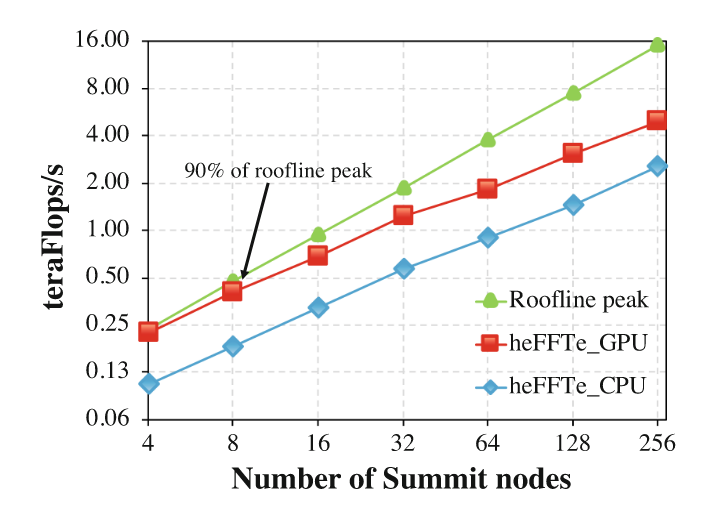
\includegraphics[width=0.5\linewidth]{figures/heFFTe.png}
    \caption{Roofline performance estimated from eq. 3 in Ref \cite{heFFTe2020} (green), heFFTe performance on a 3D FFT of size $1024^3$; using 40 MPI processes, 1 MPI/core, per node (blue); 6 MPI per node, 1 MPI/1 GPU-Volta100, per node (red). From Ref \cite{heFFTe2020}.}
    \label{fig:heFFTe}
\end{figure}


We note that the performance data of Nvidia's cuFFT was provided to us in early 2020, which was also consistent with above characterization. For $1024^3$ FFT, cuFFT can reach 0.7TF/sec on one GPU on Lassen, which is a reflection of MB, 0.7TB/sec, not the peak FP performance of 7TF/sec. In addition, the performance improvement was observed only up to 2 GPUs on a single socket, which has a higher IB than internode IB. For larger number of GPUs and/or smaller FFT grid size, performance degrade compared to the serial performance indicating the IB/MB limited nature of parallel FFT algorithm.  

In order to understand the true upper limit of 3D FFT performance on CPU-GPU hybrid architecture, {\bf Ogitsu} is in communication with Prof. Stanimire Tomov of U. Tennesee, who leads heFFTe project, and discussing about a research plan in mapping the performance of 3D FFT against FP, MB and IB values so as to develop a HPC hardware design guideline for 3D FFT algorithm. This information will be shared with the scientific and HPC communities so as to assist development of HPC architecture design suitable for their high priority software applications.

At last, we point out that there is a clear indication that the HPC community is moving towards SOC (system on chip: CPU, GPU and memory on one chip) based HPC chip similar to Apple M1, which will eliminate redundant memory space and interconnect, which, in turn, will improve the cost performance and power consumption rate of a HPC system.

